\chapter{Implementation}

\begin{comment}
Chapter 4: Implementation
The implementation details should be confined to the important, difficult or interesting aspects. Large chunks of code should be avoided, and diagrams and tables should be used to present details clearly.
\end{comment}

\plan{Limited to programming languages only}

\begin{comment}
Statement Management 
Upload
NamedEntityResolution
Suggestions ........................ 19

Prediction
MarkovChain
WeightedArithmeticMean
FiveModelSystem
Confidence

Security Considerations
AccountHijacking
PasswordSecurity
Database Security
Other
\end{comment}

This section is focused on particularly interesting or troublesome parts of implementing the design outlined in \ref{cha:design} and any usage of external libraries. As it was decided the project would be a web application\todo{Should probably mention this in design} the user interface was written in HTML \& CSS, with the interactive elements such as the graphs in JavaScript. PHP was chosen as the server side language used to process the user and the database was implemented using MySQL.

PHP was selected as the server side language because the author had extensive experience in the language, it's original intended use was web development and it is well supported. It's intention of web development means it's well coupled with HTML and provides many libraries to handle it, giving the language a significant advantage over languages such as Python and Java which can be adapted for web use. A key disadvantage of PHP is that is it weak typed which lead to some issues during development where objects of the wrong type were passed into functions. This disadvantage was considered and it was decided the advantages outweighed the disadvantages.

The project uses a PHP Framework, written by the author \todo{This doesn't make sense} called pegFramework. Using a framework has several key advantages over writing the whole system.

Frameworks:
Provide standardised code and file organisation - pegFramework has a well defined code structure, code is organised in a predefined way and split into modules
MVC - Model View Controller - using the MVC pattern with a framework ensures models (data structures), views (page contnet) and controllers are separate, improving cohesiveness and decreasing coupling.
Utilities and libraries - frameworks handle all the standard web design code, including routing, security, controllers, rendering the template and caching.

MySQL was selected as the database language because it's well supported by PHP and because it provides Natural Language Searching out of the box, which supports free-text queries and can calculate the relevance of a record in the database to a search term. This is used to power the suggestions section of the website and for user entered searches.

Server Side Libraries:

Twig - a template engine that takes collections of PHP objects and following a provided .html template build the output sent to the browser. In addition it provides caching of the generated templates and output, leading to significant speed increases for the end user.

Propel - an object relational mapping (ORM) library for PHP. Propel takes a database schema defined in XML and generates PHP objects that represent the schema which can be saved to and loaded from the database.

Less - CSS pre-processor that extends CSS, adding additional features and inheritance. `.less` files compile to `.css`

Front End

Bootstrap - framework for CSS development that provides grid and stuff

jQuery - javascript development framework that abstracts differences in browser behaviour and provides shorthands to common tasks such as ajax requests



Chosen - javascript libray to make dropdown boxes better

Highcharts - charting library for the UI

\section[Statements]{Statement Management}

\subsection{Upload}
OFX is an XML like format called SGML. PHP has inbuilt libraries for parsing XML called SimpleXML simplexml\_load\_string loads an XML file from a string. To parse the OFX, PHP attempts to parse it as an XML file and captures any exceptions. If exeptions are found it attempts to convert the SGML XML so it can be pased by PHP as per \todo{This needs completing}

%http://stackoverflow.com/questions/15735330/how-to-parse-a-ofx-version-1-0-2-file-in-php and http://www.hanselman.com/blog/PostprocessingAutoClosedSGMLTagsWithTheSGMLReader.aspx

\todo{Comparison of SGML and XML}

For each line of the SGML it trims whitespace including (x,y,z), converts the charset ot UTF-8 so it's valid in PHP and if no closing tag is found, appends a closing tag

\begin{figure}
\lstset{style=phpcolor}
\begin{lstlisting}
foreach(preg_split("/((\r?\n)|(\r\n?))/", $this->OFXContent) as $line){
        		
        	// Trim whitespace
        	$line = trim($line);
        	if ($line === '') continue;
        
        	// Convert charset to UTF-8
        	$line = iconv($charset, 'UTF-8', $line);
        	if (substr($line, -1, 1) !== '>') {
        		list($tag) = explode('>', $line, 2);
        		$line .= '</' . substr($tag, 1) . '>';
        	}
        	$buffer .= $line ."\n";
}
\end{lstlisting}
\caption{Converting SGML to XML}
\end{figure}

Having parsed the SGML into objects it can just be navigated following the specification and converted to arrays of information for each transaction, refered to as movements. These movements look like XYZ; and can then be convered into the Transaction objects most of the fields are handled automatically but dates need to be handled specifically.

QIF is handled in a different manor as there are no native libraries to parse it's format. As per the Fig. \ref{fig:qifofxformat} shown in section \ref{subsection:upload} shown in  the format is a list of individual movements, with each terminated a \^. Each field associated with an individual movement is identified with a letter, explaining the contents of that line.
% 
The field types that the project was interested in and parses are shown in Table \ref{table:qiffields}.

\begin{table}[h]
\begin{tabular}{ll}
D                  & Date           \\
T                  & Amount         \\
C                  & Cleared status \\
P                  & Payee          \\
M                  & Memo           \\
\textasciicircum   & End of entry  
\end{tabular}
\caption{QIF fields parsed by the project}
\label{table:qiffields}
\end{table}

In a similar manner to parsing the OFX files, the application loops though all the lines found in the file, switching on the identifier and sorting the information into an array representing that movement. 

\begin{figure}
\lstset{style=phpcolor}
\begin{lstlisting}
$id = substr($line, 0, 1);
$content = trim(substr($line, 1));

switch ($id) {
	case '^': // End of entry
		$this->movements[] = $newMovement;
		$newMovement = array();
		break;
		
	case 'T': 	// Amount
		$newMovement["value"] = floatval(preg_replace("/[^0-9.-]/", "", $content));
		break;
		
	case 'D': 	// Date
		$newMovement["date"] = $content;
		break;
		
	// etc ...
\end{lstlisting}
\caption{Parsing QIF transactions using the line identifier}
\end{figure}

As outlined in section \ref{subsection:upload} the conversion from the array to a Transaction object is slightly more involved due to unknown date format. To implement this in PHP, before beginning the conversion, all movements are tested against two regular expressions (regex), representing the possible formats of the dates, which are visualised as graphs in Fig. \ref{fig:regex-dmy} and \ref{fig:regex-mdy}. 
%
Having considered all the movements found in the file, the application has either decided on one of the date formats or prompts the user to decide the appropriate format, as seen in Fig. \ref{fig:dateformat-prompt}.

\begin{figure}
\lstset{style=phpcolor}
\begin{lstlisting}
$dmy = true;
$mdy = true;
foreach($this->getMovements() as $movement)
	if(!preg_match('#(0[1-9]|[12][0-9]|3[01])[-/](0[1-9]|1[012])[-/](19|20|21)?\d\d#', $date))
		$dmy = false;
	
	if(!preg_match('#(0[1-9]|1[012])[-/](0[1-9]|[12][0-9]|3[01])[-/](19|20|21)?\d\d#', $date))
		$mdy = false;
\end{lstlisting}
\caption{Identifying the date format using regular expressions}
\end{figure}

\begin{figure}[h]
    \centering
    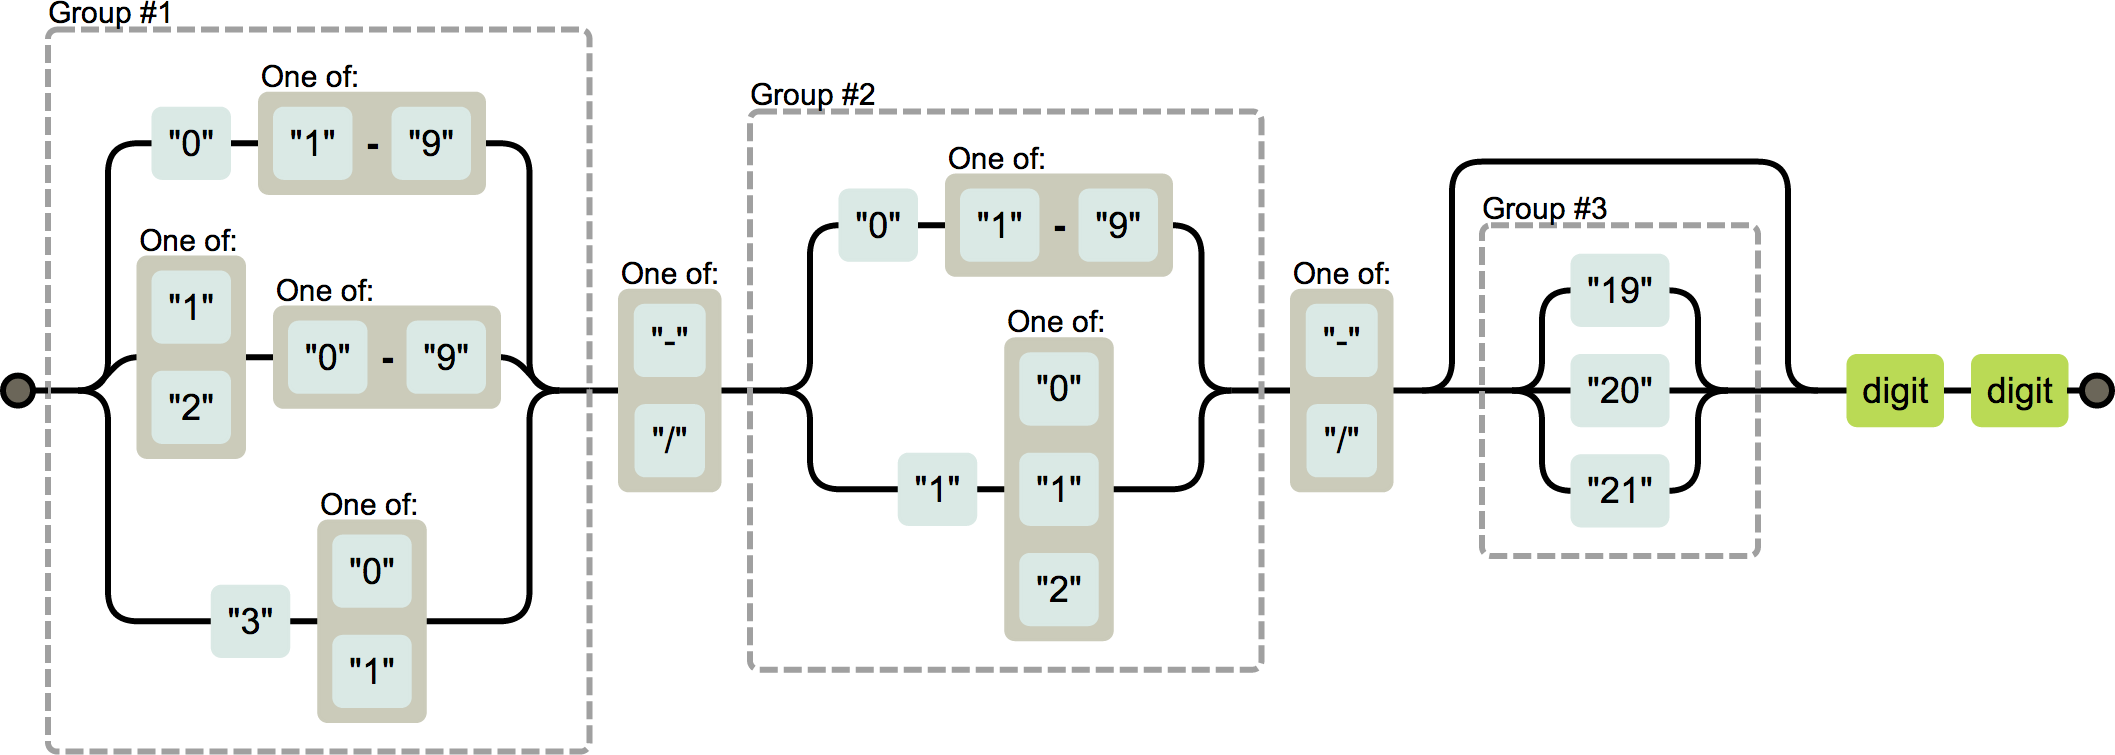
\includegraphics[width=\textwidth]{implementation/regex-dmy}
    \caption[Regular expression used to match d-m-Y]{Railroad diagram of the regex used to match format d-m-Y}
    \label{fig:regex-dmy}
\end{figure}

\begin{figure}[h]
    \centering
    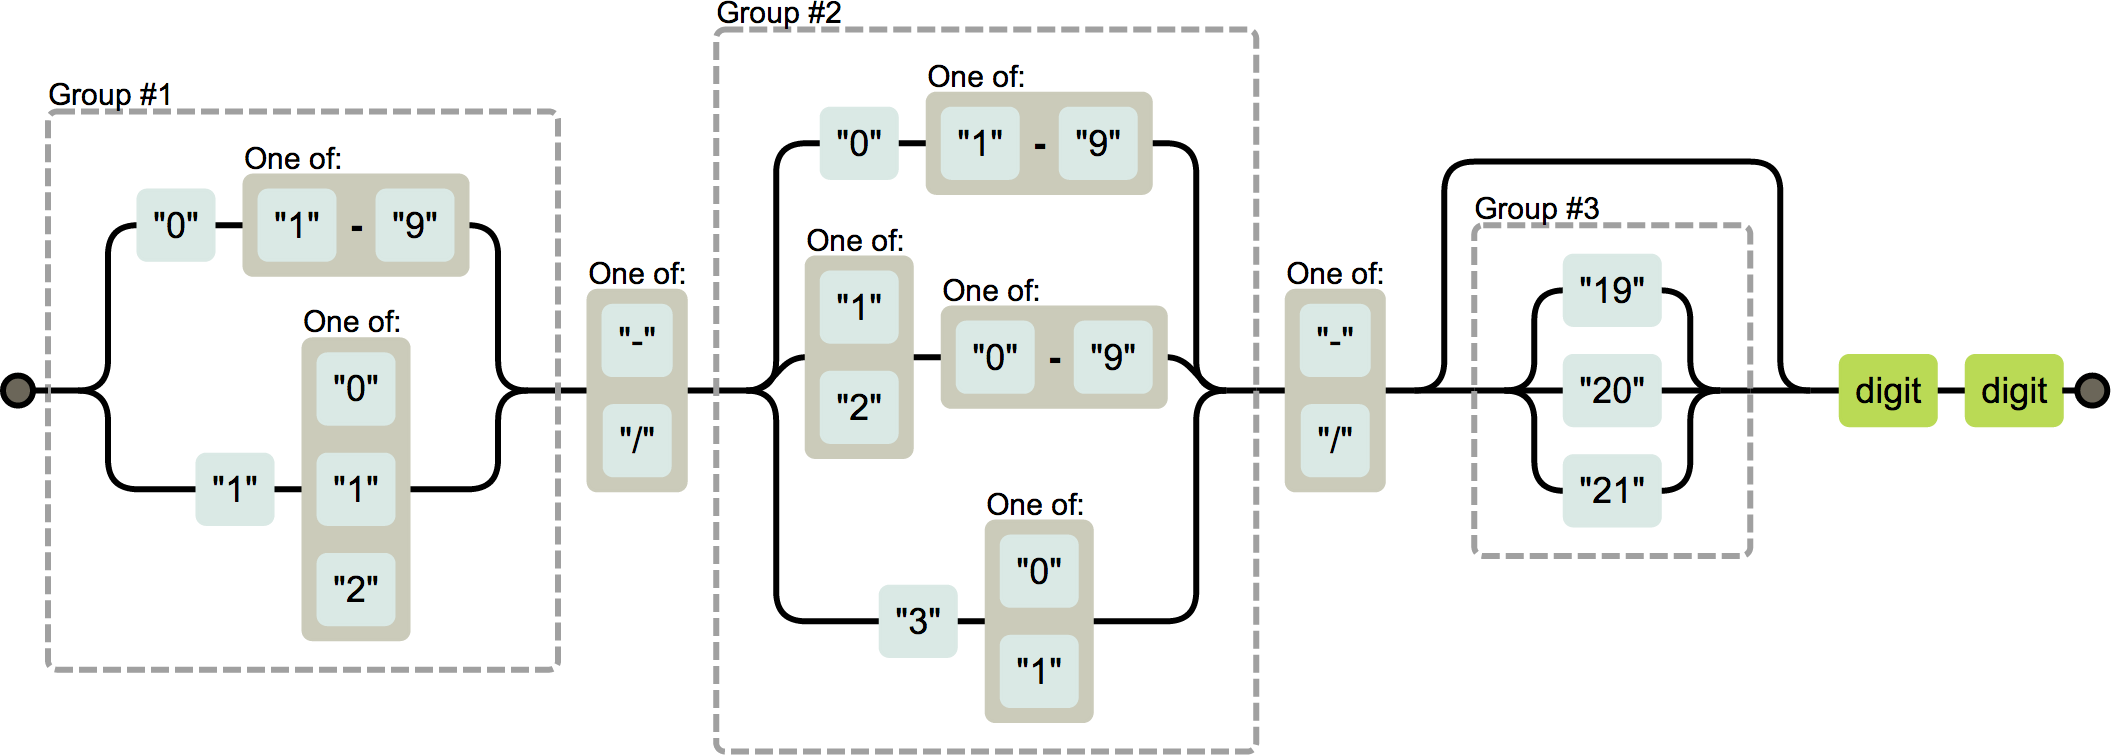
\includegraphics[width=\textwidth]{implementation/regex-mdy}
    \caption[Regular expression used to match m-d-Y]{Railroad diagram of the regex used to match format m-d-Y}
    \label{fig:regex-mdy}
\end{figure}

\begin{figure}[h]
    \centering
    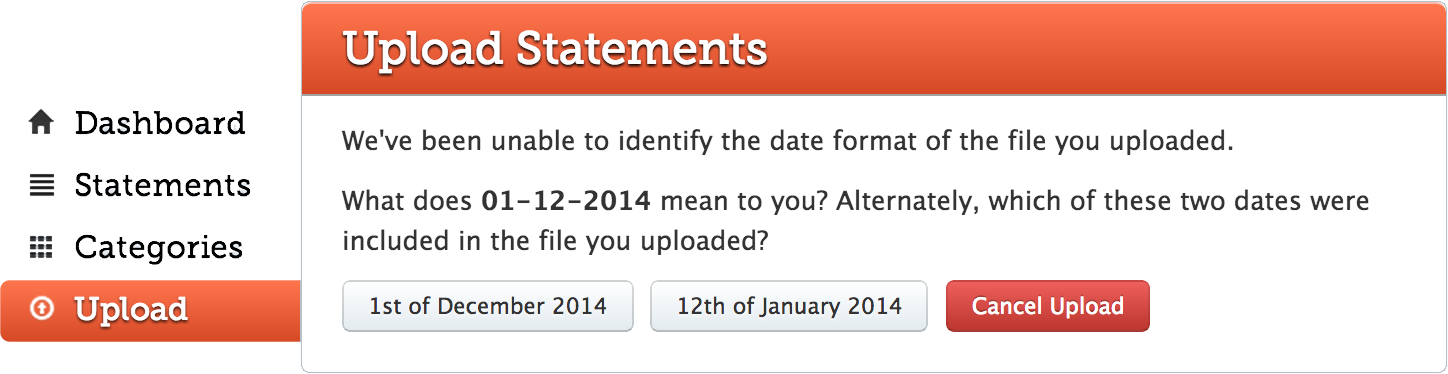
\includegraphics[width=0.70\textwidth]{implementation/dateformat-prompt}
    \caption{UI Prompt when the application is unable to decide an upload's date format}
    \label{fig:dateformat-prompt}
\end{figure}

\subsection{Named Entity Resolution}
The implemented the mapping architecture outlined in the design, the majority of the named entity resolution is done in the \lstinline{setTransactor} method of the Transaction object, which is called when setting the name of transactor for a each transaction found in the uploaded file.   
% 
The method performs three key actions, tidying the string, removing common notation added by banking institutions and checking the database for known user and global transactors, otherwise creating a new one.
% 
To avoid unnecessary duplication in the mappings table the \gls{transactor} names are normalised before checking for an existing name, this normalisation was added to combat the various different ways which banks store the transactor names which were discovered during testing. The modifications included: padding with spaces, replacing spaces with underscores/tabs, or including non alphanumeric letters; some examples are shown in Table \ref{table:cleaningstrings}.
%
Having normalised the input, the next step was to remove any numeric identifiers which had been added and move that detail to another field. Examples of such identifiers included store id's for shops with multiple outlets and account numbers for transfers between accounts, if this detail wasn't removed a separate mapping would be created for transactions referencing the same entity, leading to unnecessary duplication. The identifiers were removed using a regex, expressed in Fig. \ref{fig:regex-transactor} which only captures numbers found at the end of the string requiring at least two digits, these additional constraints were added to preserve \glspl{transactor} with numbers in their name, such as \inlinetext$H3G$ and \inlinetext$SUPERMERCADO 3$.
%
The final step checks for existing \glslink{globaltransactor}{GlobalMapping} or \glslink{usertransactor}{UserMapping} objects in the database and if found associates that mapping with this transaction. If neither mapping's are found a new \glslink{usertransactor}{UserMapping} object is created, persisted and associated with the transaction. Differing from the original plan, fuzzy matching\footnote{ Finding strings that approximately rather than exactly match} of the transactor name when searching for existing transactors is not performed as this functionality was moved to the suggestion wizard.
%
The full code for the `setTransactor` method is shown in Fig. \ref{fig:settransactor}.

\lstset{language=textwithspaces,style=showspaces}
\begin{table}[h]
\centering
\begin{tabular}{ll}
Raw Transactor Name & Occurrences \\
\inlinetext$TESCO STORES 5128$   & 87         \\
\inlinetext$TESCO STORES 2977$   & 68         \\
\inlinetext$TESCO_STORES$        & 14         \\
\inlinetext$SACAT MARKS    AND$  & 33         \\
\inlinetext$SACAT MARKS  AND$    & 16         \\
\inlinetext$WILKINSON $          & 22         \\
\inlinetext$WILKINSON$           & 8          \\        
\inlinetext$TO A/C 00000000$\footnote{Account number removed} & 2  
\end{tabular}
\caption{Examples of the raw transactor names found on uploaded statements}
\label{table:cleaningstrings}
\end{table}

\begin{figure}[h]
    \centering
    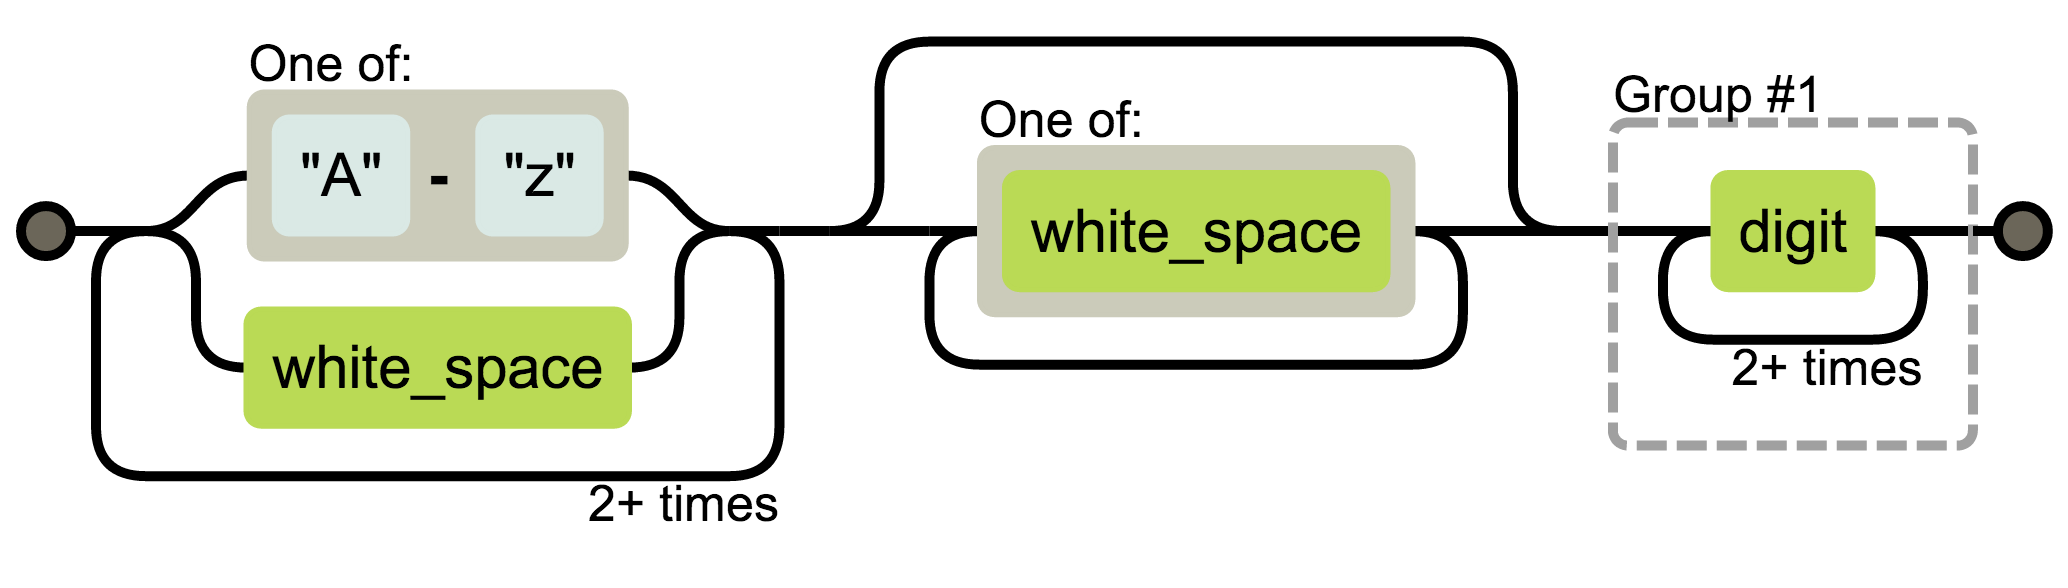
\includegraphics[width=\textwidth]{implementation/regex-transactor}
    \caption[Regular expression used to match the transactor name]{Railroad diagram of the regex used to tidy the transactor name}
    \label{fig:regex-transactor}
\end{figure}

\subsection{Suggestion Wizard}
The suggestion wizard (Fig \ref{fig:suggestion-wizard}) was added to the project in response to observations during lab usability testing. Originally the suggestions were only found on each unmapped transactors page (Fig. \ref{fig:view-reference-suggestions}) to speed up the process of mapping a reference to an existing transactor.  Users appeared to spend a lot of time manually categorising each individual transactor by searching their statement for an unknown transactor, opening that transactors details and then filling in the appropriate forms or clicking on a suggestion, following an activity diagram similar to Fig. \ref{fig:transactor-mapping-activity}.

\begin{figure}[h]
    \centering
    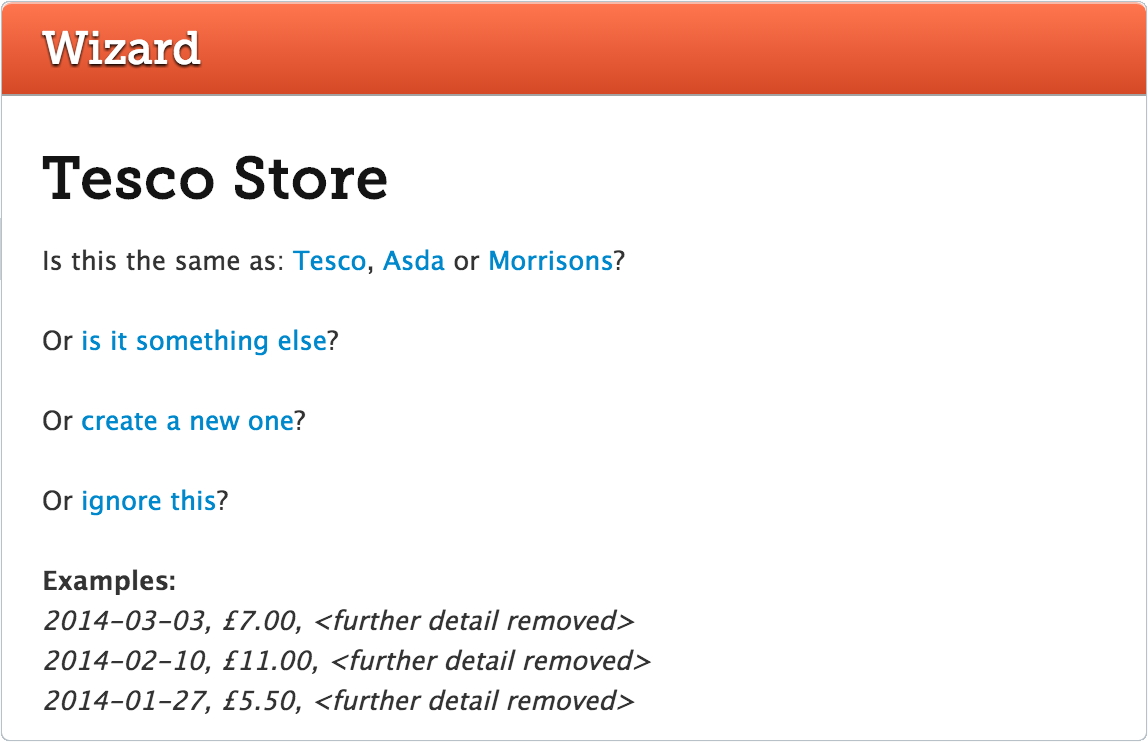
\includegraphics[width=0.75\textwidth]{implementation/suggestion-wizard}
    \caption[Suggestion wizard UI]{Suggestion wizard UI\protect\footnotemark}
    \label{fig:suggestion-wizard}
\end{figure}
\footnotetext{Potentially personally identifiable information removed}

\begin{figure}[h]
    \centering
    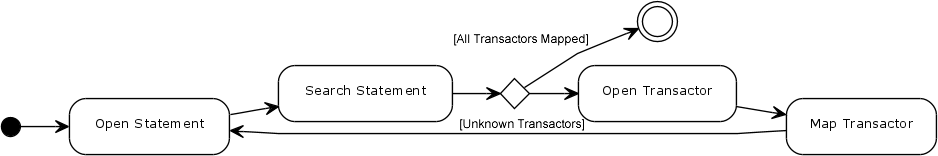
\includegraphics[width=\textwidth]{implementation/transactor-mapping-activity}
    \caption{Activity diagram for mapping individual transactors}
    \label{fig:transactor-mapping-activity}
    
    \begin{comment}
(start)->(Open Statement)->(Search Statement)-><a>->(end)
<a>->(Open Transactor)->(Map Transactor)->(Open Statement)
    \end{comment}
\end{figure}

\begin{figure}[h]
    \centering
    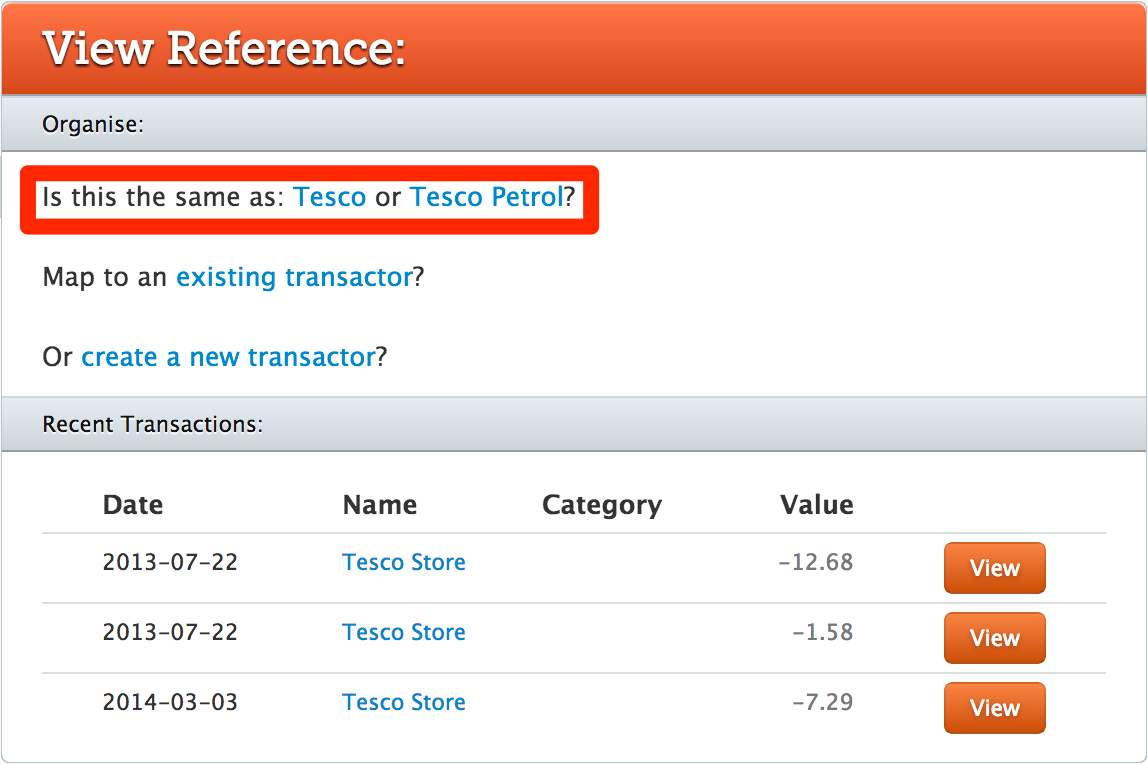
\includegraphics[width=0.75\textwidth]{implementation/view-reference-suggestions}
    \caption{Suggestions shown on the Transactor (reference) page}
    \label{fig:view-reference-suggestions}
\end{figure}

The wizard was designed to streamline and speed up this process as well as making it easier for the user to follow. Each unmapped transactor is displayed in turn, starting with the one with the most transactions (encouraging the user to map the ones they shop at more often first). On each step, the user can; follow the suggestions, manually map the reference to an existing transactor, create a new transactor or ignore the reference for now. A step-by-step view of this process is shown in section \ref{subsection:suggestion-wizard-walkthrough}.

During the process feedback is displayed to the user using notifications that appear over the wizard and are coloured according to validation style convention, with red warning of an error and green confirming success (Fig. \ref{fig:suggestion-notification}). 
%
The notifications themselves were implemented using the PNofity javascript library for jQuery which provides an API for managing alerts send to the user. PNotify was chosen as it had native support for bootstrap styles, which were already being used for the projects UI, and it was open source licensed under the GPL\footnote{GNU General Public License \parencite{gnu2007license}} \parencite{huber2014potify}.

\begin{figure}[h]
    \centering
    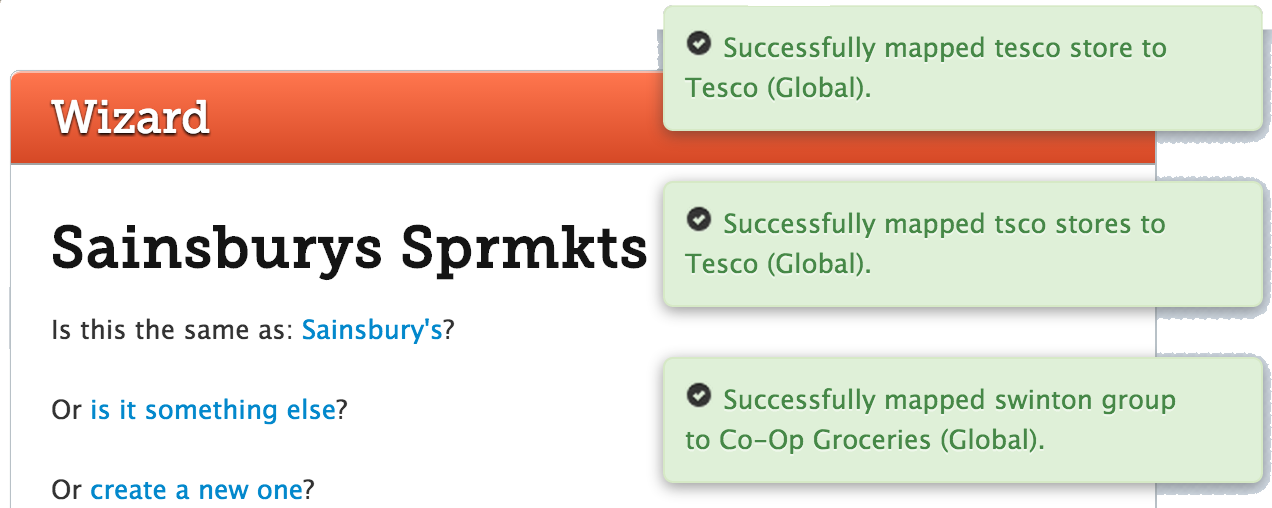
\includegraphics[width=0.75\textwidth]{implementation/suggestion-notification}
    \caption{Notifications shown during the suggestion wizard}
    \label{fig:suggestion-notification}
\end{figure}

By following the wizard users are able to quickly map the majority of their transactions in an easy to follow way, as can be shown by the activity diagram in Fig. \ref{fig:suggestion-wizard-activity}.

\begin{figure}[h]
    \centering
    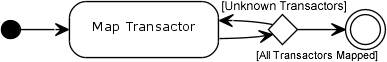
\includegraphics[width=0.6\textwidth]{implementation/suggestion-wizard-activity}
    \caption{Mapping transactors using the suggestion wizard activity diagram}
    \label{fig:suggestion-wizard-activity}
    
    \begin{comment}
(start)->(Map Transactor)-><a>->(end)
<a>->(Map Transactor)
    \end{comment}
\end{figure}

The wizard is powered by Ajax\footnote{Asynchronous JavaScript and XML}, which sends requests to a backend RESTful API which proves access to the unmapped transactors found for the user. The requests and responses are sent as JSON\footnote{JavaScript Object Notation} which is supported natively by both PHP and JavaScript. A GET request to \lstinline{/ajax/transactor/suggestions} returns a collection of unmapped transactors including associated examples which are then added to the UI using JavaScript.
%
Mapping (including following a suggestion) and creating a new transactor are both handled by POST requests to the same API. Mapping sends a request to \lstinline{/ajax/transactor/map} containing the ID of the user mapping and global mapping  and creation sends a request to \lstinline{/ajax/transactor/create} including the user mapping ID to associate with the new transactor. 
%
Examples of the JSON communication are shown in Fig. \ref{fig:json-examples}.

On the backend, all JSON serialisation is handled by implementing the \inlinephp{JsonSerializable} interface on all objects that need to be JSON encoded. This allows the native function \inlinephp{json_encode(\$object)} to correctly encode the object into JSON using the data returned by the abstract method `jsonSerialize` defined in the interface. The final inheritance diagram for the mapping, transactor and transaction objects is shown in Fig. \ref{fig:mapping-inheritance-diagram}.

\begin{figure}[h]
    \centering
    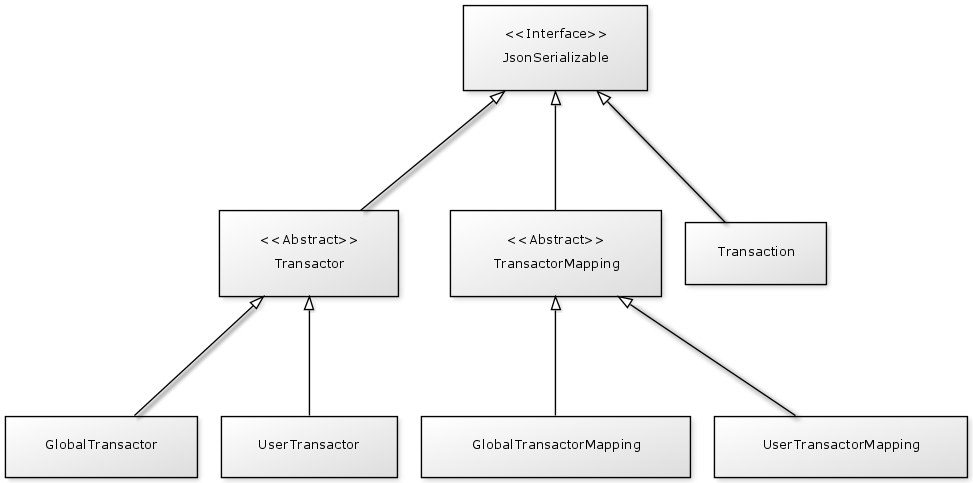
\includegraphics[width=\textwidth]{implementation/json-serializable}
    \caption{Inheritance diagram of JsonSerializable objects}
    \label{fig:mapping-inheritance-diagram}
    
    \begin{comment}
[<<Interface>> JsonSerializable]^-[<<Abstract>> Transactor]
[<<Interface>> JsonSerializable]^-[<<Abstract>> TransactorMapping]
[<<Interface>> JsonSerializable]^-[Transaction]
[<<Abstract>> TransactorMapping]^-[UserTransactorMapping]
[<<Abstract>> TransactorMapping]^-[GlobalTransactorMapping]
[<<Abstract>> Transactor]^-[UserTransactor]
[<<Abstract>> Transactor]^-[GlobalTransactor]
    \end{comment}
\end{figure}

\subsubsection{The Suggestions} \label{sec:suggestionimplementation}
The suggestions are made by searching for known global mappings, user mappings, global transactors and user transactors\footnote{In the order of preference} that are similar to the reference name a suggestion is being made for. This is done using the Natural Language Full-Text Search functions provided by MySQL. These functions, including \inlinesql$MATCH$, use a Vector Space Model to rank the relevance of a field relative to the input and signify this relevance using a decimal number, which means it can be treated as a standard field by the database and used to order the results.  \parencite{mysql2014searches}. 

When searching for suggestions the application finds the five most relevant mappings or transactors, according to full text search, loads those objects from the database using the ORM. As the ORM tool uses doesn't have support for full text search a raw SQL query was written that uses PDO's\footnote{PHP Data Objects extension for accessing databases} prepared statements functionality to send the parameters to the database server, avoiding SQL injection. The query for finding global transactor mappings as part of the \inlinephp{GetCloseTransactorMappings} method in the GlobalTransactorMappingPeer class is shown in Fig. \ref{fig:sql-match-query}, where \inlinesql{:identifier} is replaced by the server with the passed parameters.

\begin{figure}
\centering
\begin{lstlisting}[language=sql]
SELECT *, MATCH(:nameColumn) AGAINST (:name) AS 'score'
FROM :tableName
	WHERE :transactorID IS NOT NULL
	HAVING `score` > :minScore OR :nameColumn = :name
ORDER BY `score` DESC
LIMIT 5
\end{lstlisting}
\caption{SQL Query selecting similar mappings or transactors using PDO}
\label{fig:sql-match-query}
\end{figure}

\section{Prediction}
The key difficulty of implementing the prediction functionality was designing a data structure that allowed predictions to be read by column or by row in order to generate the table output shown in Fig. \ref{fig:imp-categories-overview}. Ordinarily a multidimensional array or a dictionary of dictionaries would be used, however in this case it must be possible to access the data by subcategory as well as by month or date.
%
In order to allow accessing the data by month, category and subcategory as well as being able to generate totals the data structure shown in Fig. \ref{fig:prediction-inheritance-diagram} was used. The TransactionCollection interface defines three methods, \inlinephp{getTotalValue()}, \inlinephp{getTransactions()} and \inlinephp{addTransaction(Transaction)}. Using this interface means that each level of the data structure can be treated in exactly the same way and has the advantage that the entire PersonalBudget object can be passed to the template engine with no controller logic or pre-calculation. Transactions are added to the PersonalBudget object and at each layer of the data structure organised into the correct collection automatically. When getting the transactions from any collection, the object calls the get \inlinephp{getTransactions()} method on any sub-collection instances it holds and returns an intersection of the results.

\begin{figure}[h]
    \centering
    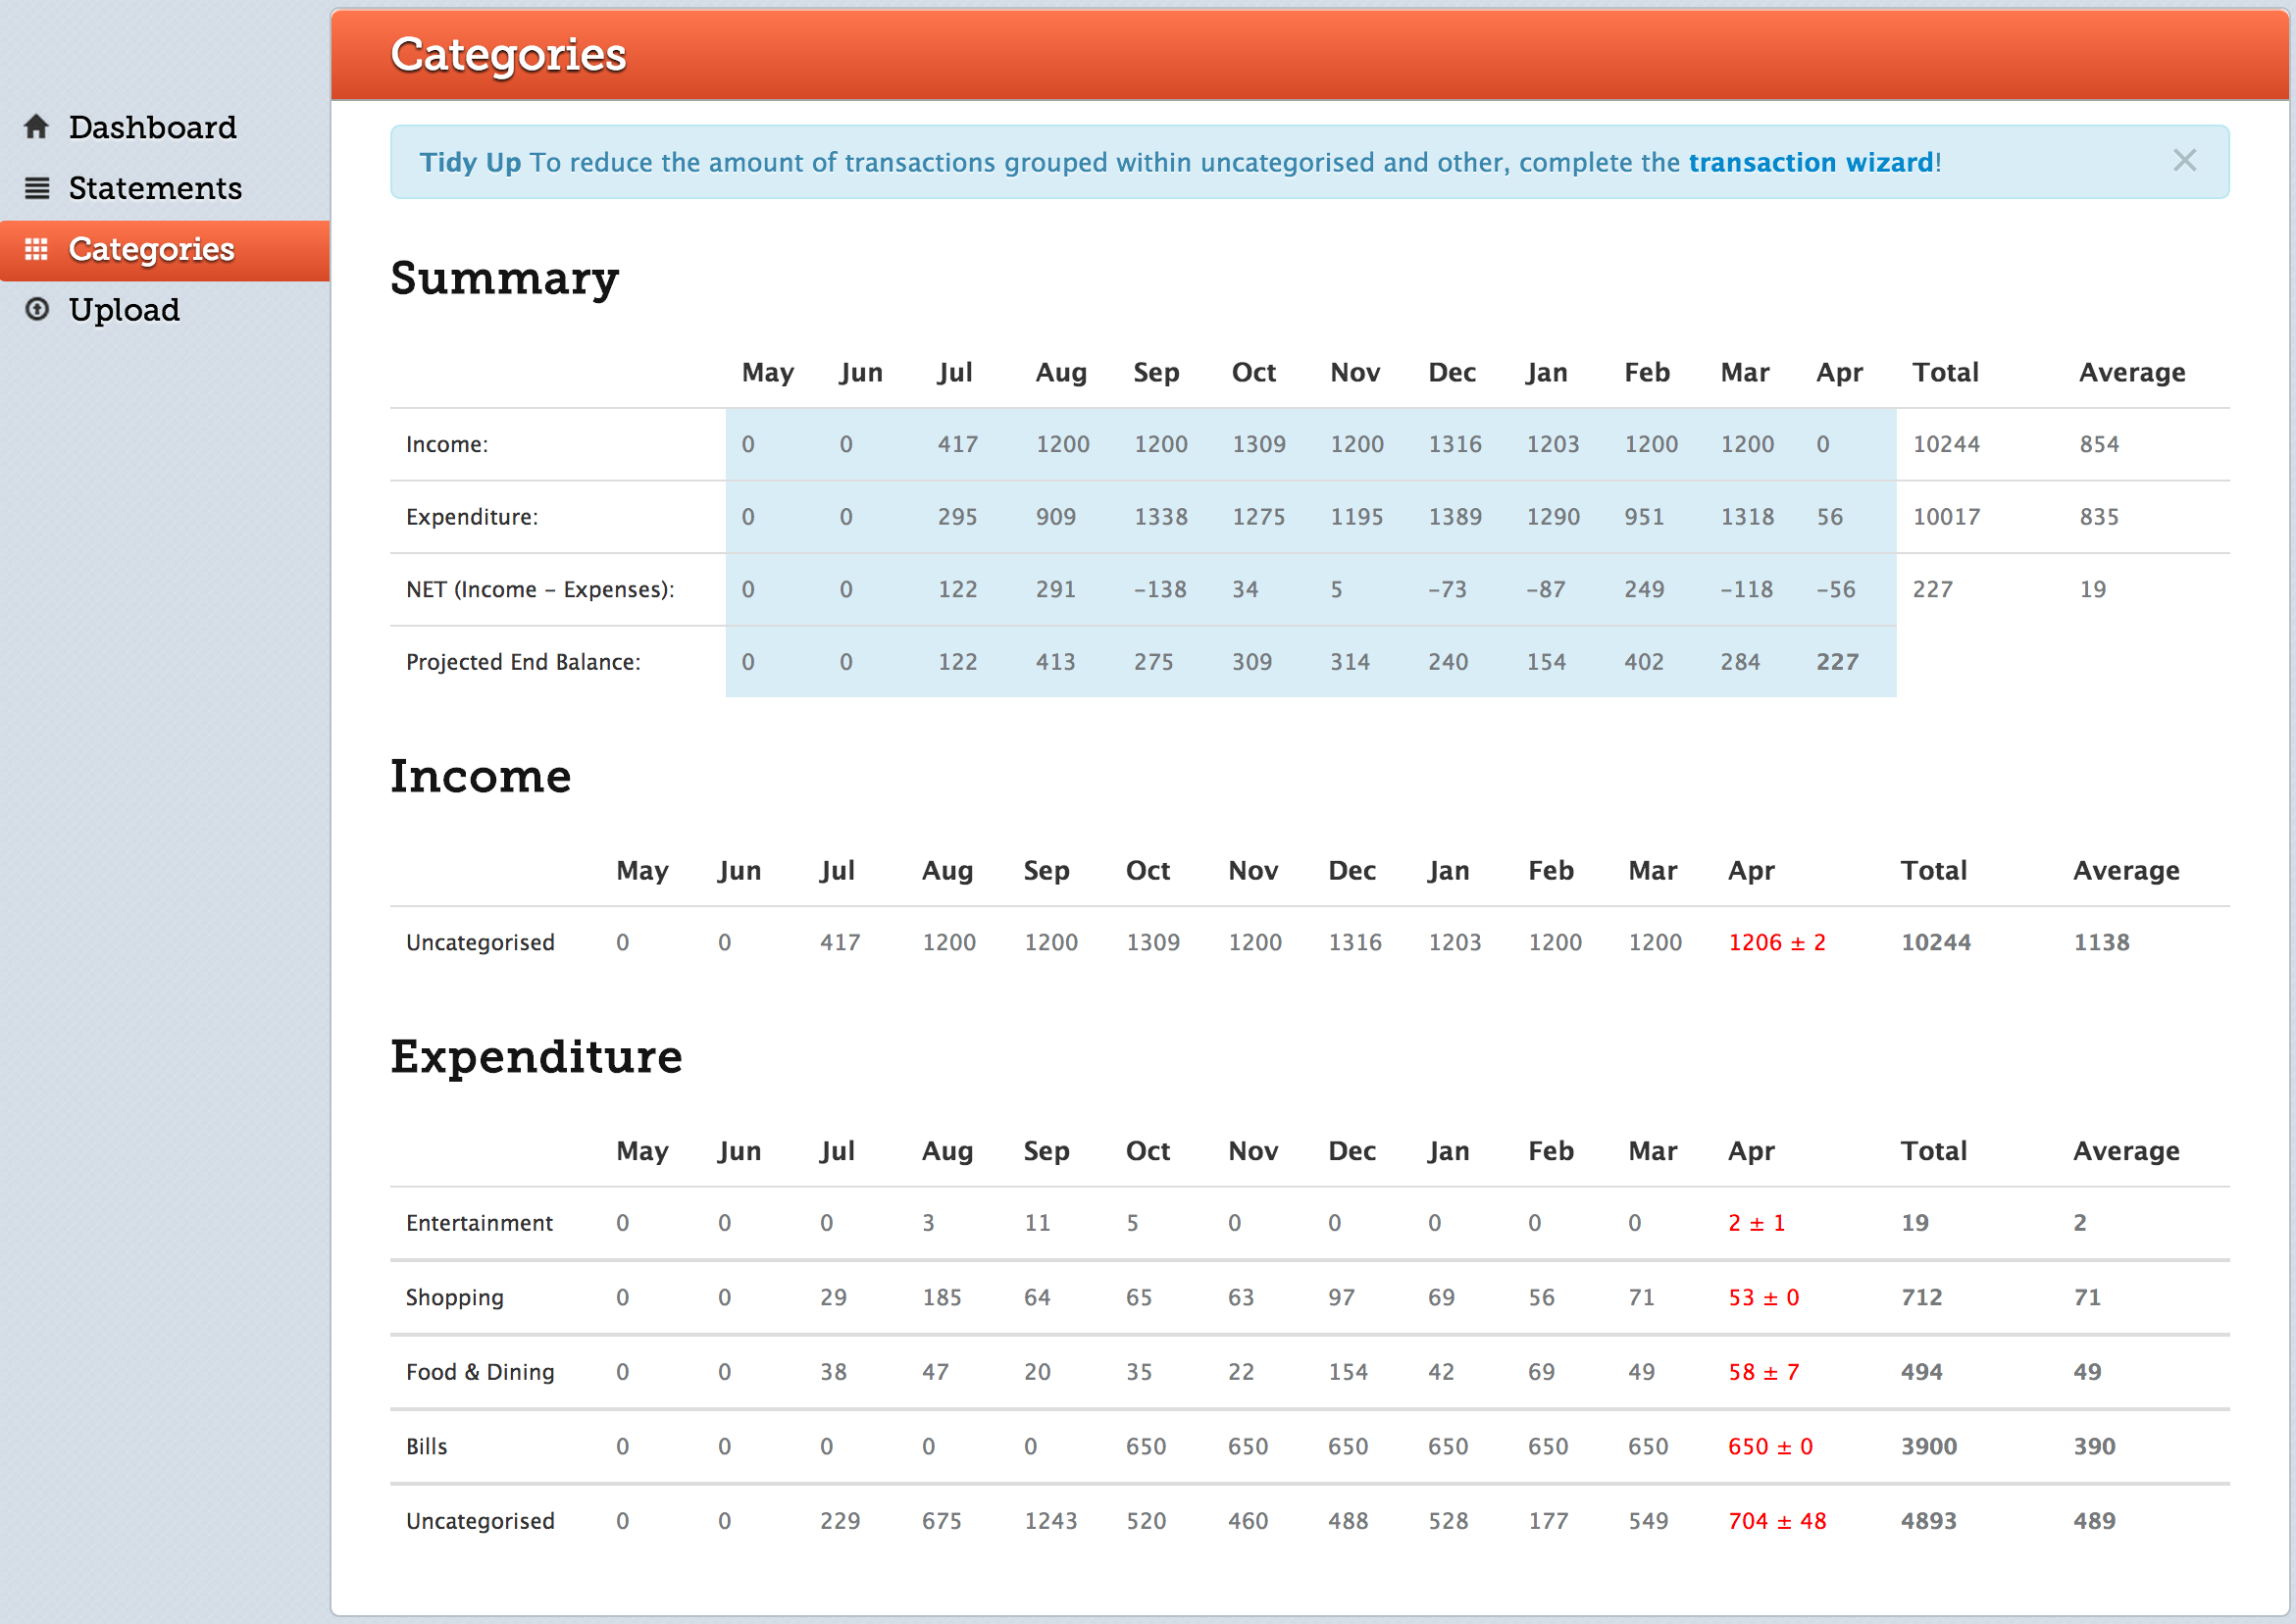
\includegraphics[width=0.75\textwidth]{implementation/categories-overview-2}
    \caption{Activity diagram for mapping transactors using the suggestion wizard}
    \label{fig:imp-categories-overview}
\end{figure}

\begin{figure}[h]
    \centering
    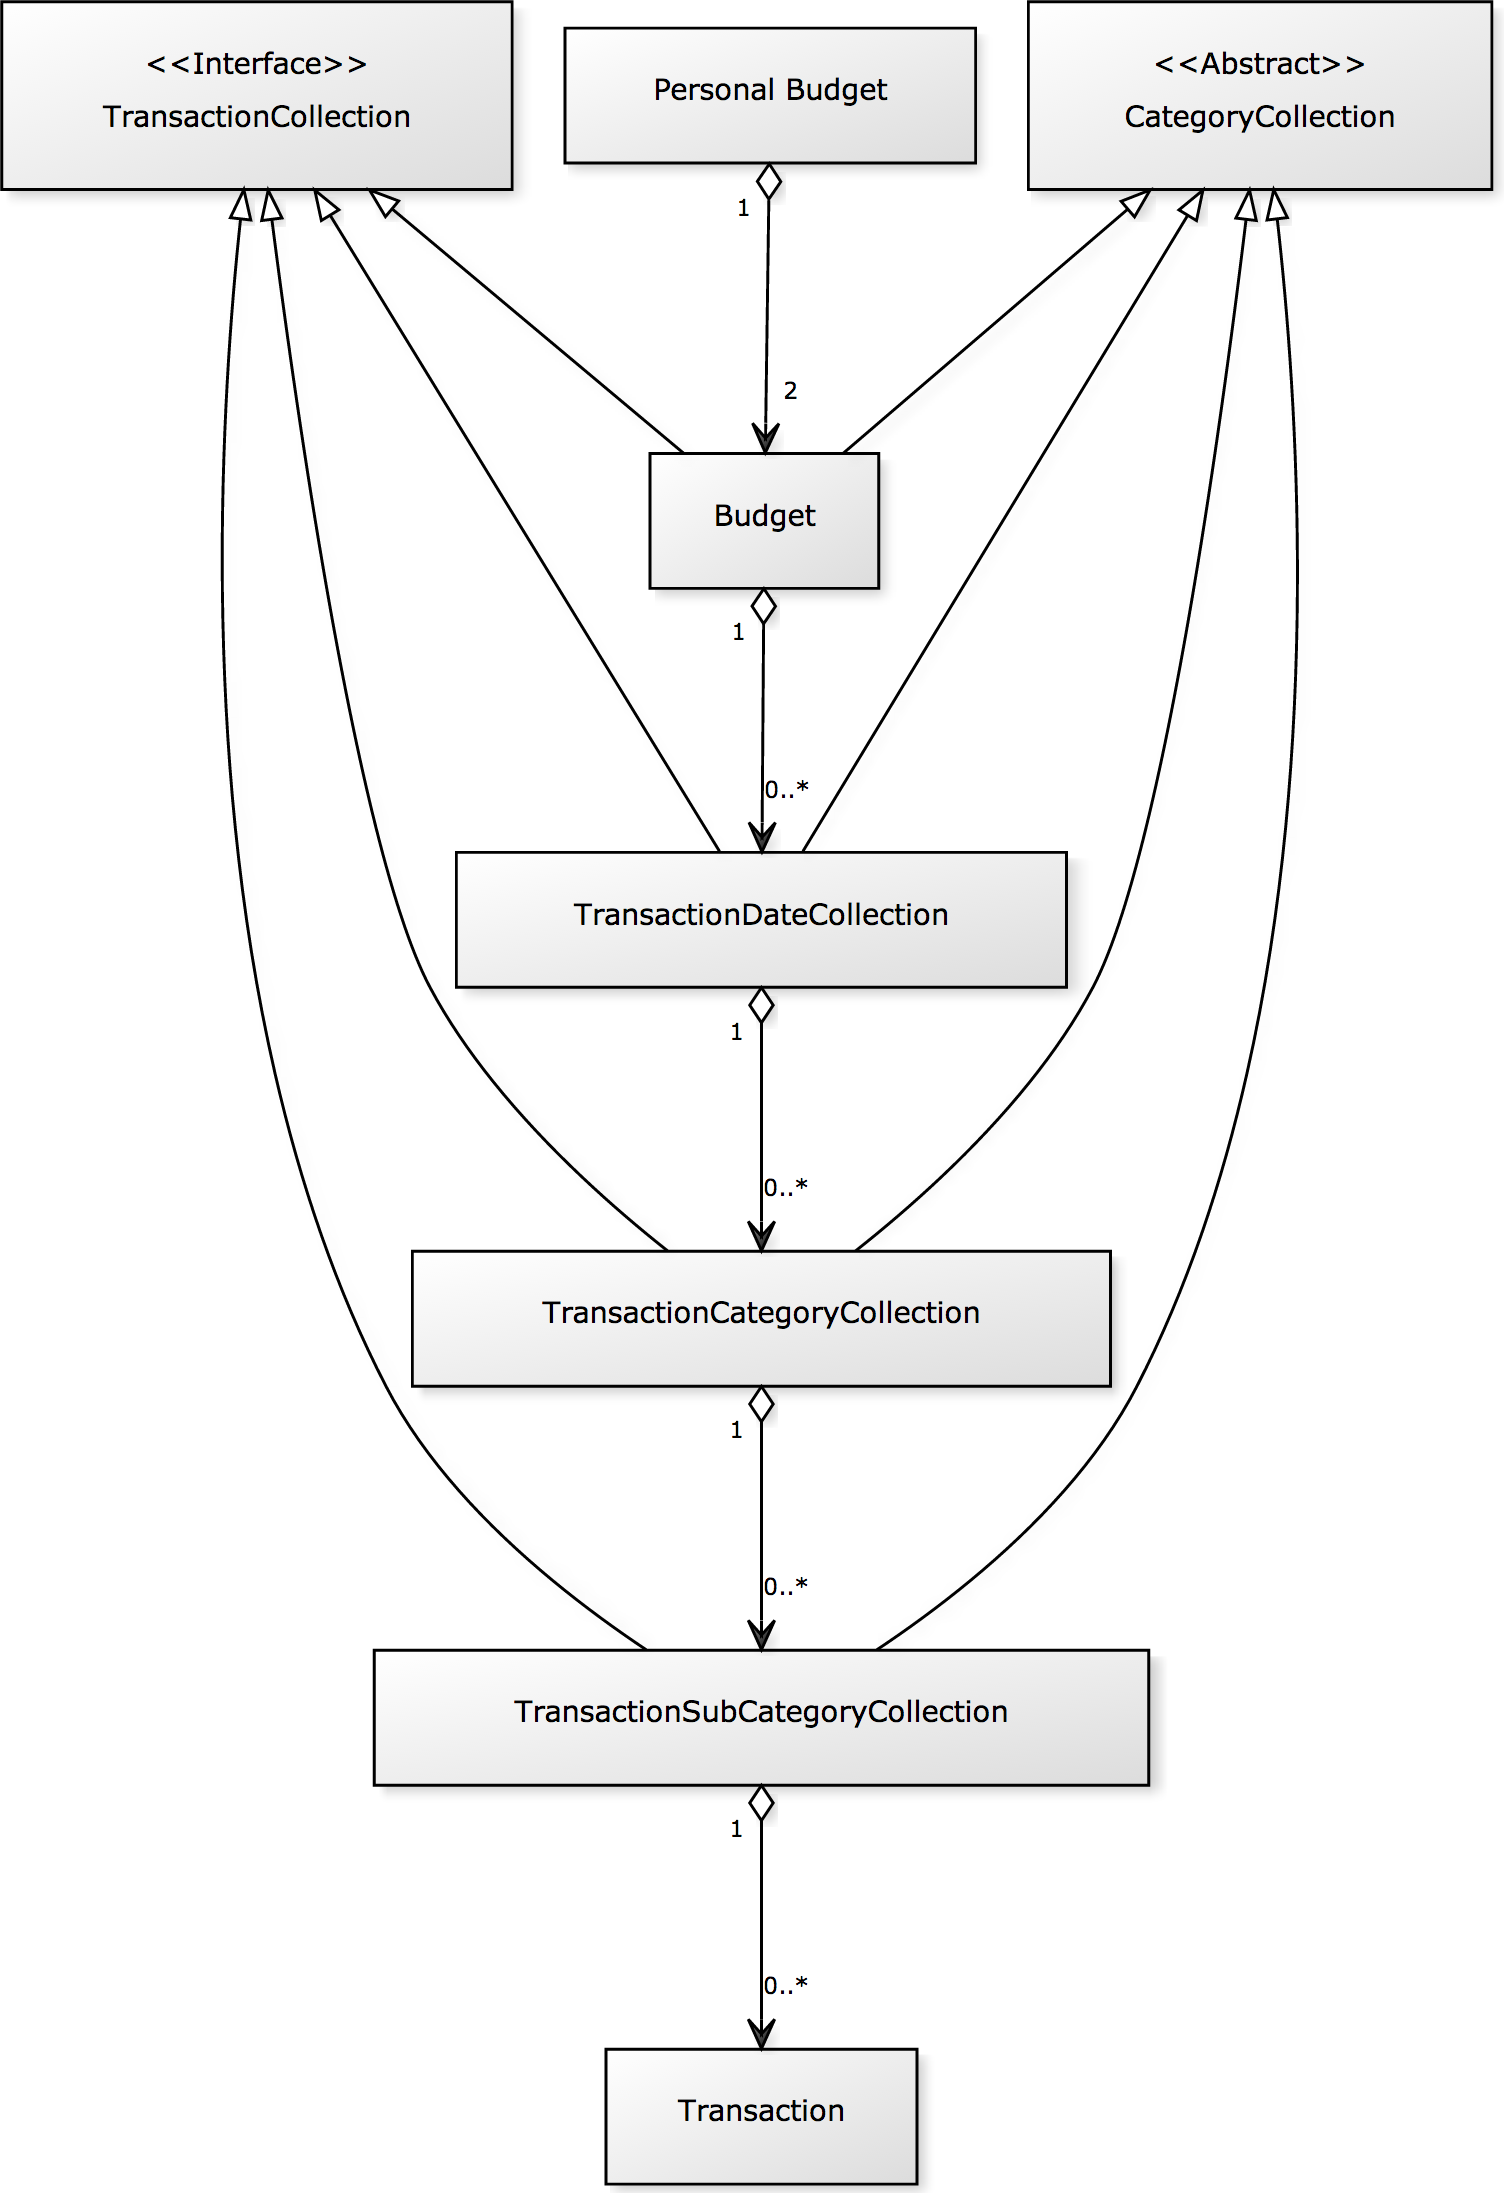
\includegraphics[width=0.75\textwidth]{implementation/mapping-inheritance-diagram}
    \caption{Data structure for storing a Personal Budget by date and (sub)category}
    \label{fig:prediction-inheritance-diagram}
    
    \begin{comment}
[PersonalBudget]<>1-2>[Budget]
[<<Abstract>> CategoryCollection]^-[Budget]
[<<Interface>>;TransactionCollection]^-[Budget]
[<<Abstract>>;CategoryCollection]^-[TransactionDateCollection]
[<<Interface>>;TransactionCollection]^-[TransactionDateCollection]
[Budget]<>1-0..*>[TransactionDateCollection]
[<<Abstract>>;CategoryCollection]^-[TransactionCategoryCollection]
[<<Interface>>;TransactionCollection]^-[TransactionCategoryCollection]
[TransactionDateCollection]<>1-0..*>[TransactionCategoryCollection]
[<<Abstract>>;CategoryCollection]^-[TransactionSubCategoryCollection]
[<<Interface>>;TransactionCollection]^-[TransactionSubCategoryCollection]
[TransactionCategoryCollection]<>1-0..*>[TransactionSubCategoryCollection]
[TransactionSubCategoryCollection]<>1-0..*>[Transaction]
    \end{comment}
\end{figure}

The Budget object (representing expenditure or income) provides the \inlinephp{getCategoryPrediction()} method which takes a month and a category and returns the systems prediction for that month. It's this method that builds and samples from the Markov Chain Models, calculates the Weighted Arithmetic Mean, and chooses the Weighting Model which provides the least absolute error for the historical data in order to make the prediction. The class also calculates the confidence interval which is displayed in the UI.

The logic for these steps is split into separate classes to improve cohesion and the overall process is shown in Fig \ref{fig:prediction-activity}. \todo{Fix}

\begin{figure}[h]
    \centering
    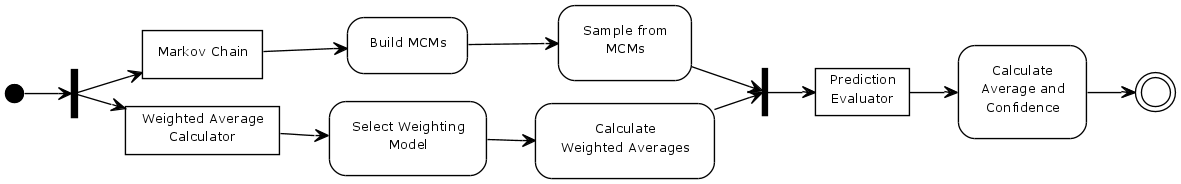
\includegraphics[width=\textwidth]{implementation/prediction-activity}
    \caption{System activity diagram when calculating the prediction a given category in a future month}
    \label{fig:prediction-activity}
    
    \begin{comment}
(start)->|a|
|a|->[Markov Chain]->(Build MCMs)->(Sample from MCMs)->|b|
|a|->[Weighted Average Calculator]->(Select Weighting Model)->(Calculate Weighted Averages)->|b|
|b|->[Prediction Evaluator]->(Calculate Average and Confidence)->(end)
    \end{comment}
\end{figure}

In order to build the Markov Chain Model the TransactionMarkovChain object takes an list of Transaction objects and counts the months where a transaction occurs, storing this in an associative array. This matrix is read to generate a transition table which represents the amount of time a transaction as transitioned from occurring to not occurring and visa-versa. This transition table can be converted to a transition matrix which represents the probability of such a transition occurring. An example transition table and matrix for a one of purchase are shown in Table \ref{table:transition-matrix}.
%
Considering whether or not a transaction occurred in the previous month, a sample is taken from the matrix. For example, if example event occurred last month for the probability of the event occurring next month given that it occurred last month is $0.00$ and so there is a 0\% chance the system will predict the event will occur next month. This process of sampling is repeated up to $10,000$ times for each transaction in under one second and the list of predictions is returned to the Budget class.

\begin{table}[!htb]

    \begin{minipage}{0.4\linewidth}
      \centering
        \begin{tabular}{lll}
        \#           & Didn't Occur & Occurred \\
        Didn't Occur & 10           & 1       \\
        Occurred     & 1            & 0      
        \end{tabular}
        \caption{Transition table for a one off purchase}
    \end{minipage} 

    \begin{minipage}{0.4\linewidth}
      \centering
        \begin{tabular}{lll}
        \#           & Didn't Occur & Occurred \\
        Didn't Occur & 0.91         & 0.09       \\
        Occurred     & 1.00         & 0.00     
        \end{tabular}
        \caption{Transition matrix for a one off purchase}
    \end{minipage}
    
    \label{table:transition-matrix}
    
\end{table}

Having decided whether or not a transaction will occur the Budget class uses an instance of \inlinephp{TransactionWeightedAverageCalculator} to estimate how much money would be transferred if a transaction occurs. The weighted average calculator takes a list of Transaction objects and returns an associative array containing the weighted average for each transactor. To calculate the weighted averages the calculator first selects the best weighting model for the users spending pattern in the specified category and uses the selected function to calculated the averages for each transactor in the category. \todo{Needs fixing}.

Combining the output of the MCM's and the weighted average calculator the produces the systems expenditure prediction for the considered category, Table \ref{table:predictions-combined}. This is calculated for each sample taken from the MCM and the results are passed to an instance of the PredictionEvaluator to produce an average and confidence interval, which is ultimately displayed on the UI.

\begin{table}[h]
\centering
\begin{tabular}{llll}
Transactor  & Prediction & Weighted Average                   & Total        \\
Tesco       & No         & £33                                & £0           \\
Sainsbury's & Yes        & £65                                & £65          \\
Amazon      & No         & £3                                 & £0           \\
Argos       & No         & £17                                & £0           \\
            &            & \multicolumn{1}{r}{\textbf{Total}} & \textbf{£65}
\end{tabular}

\label{table:predictions-combined}
\caption{Combination of the samples from the MCM and the weighted averages}
\end{table}

\section[Security]{Security Considerations}
The security considerations outlined in section \ref{section:security}, were implemented throughout the project including site-wide SSL, password entropy requirements, password salting and hashing and personal identifiable information encryption. In addition the application implements additional protection against account hijacking and login throttling to reduce the overall effectiveness of brute force attacks. 

An overview of the techniques used during login and on every page request is shown in Fig. \ref{fig:login-security} and \ref{fig:page-request-security}.

\begin{figure}[h]
    \centering
    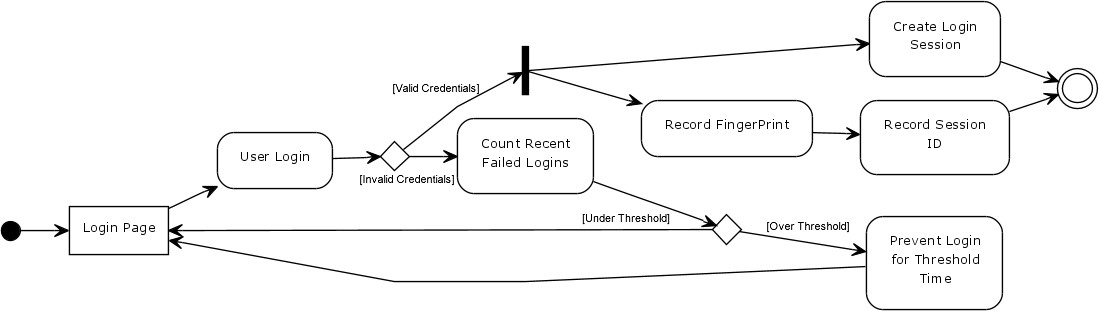
\includegraphics[width=\textwidth]{implementation/login-security}
    \caption{Steps performed during a user login}
    \label{fig:login-security}
    
    \begin{comment}
(start)->[Login Page]->(User Login)-><a>
<a>->|b|
<a>->(Count Recent Failed Logins)-><d>
<d>->(Prevent Login for Threshold Time)->[Login Page]
<d>->[Login Page]
|b|->(Create Login Session)->(end)
|b|->(Record FingerPrint)->(Record Session ID)->(end)
    \end{comment}
\end{figure}

\begin{figure}[h]
    \centering
    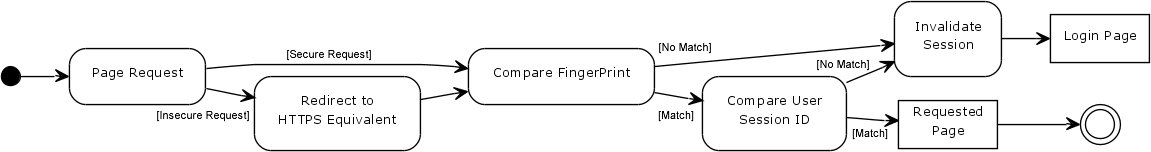
\includegraphics[width=\textwidth]{implementation/page-request-security}
    \caption{Steps performed during every page load request}
    \label{fig:page-request-security}
    
    \begin{comment}
(start)->(Page Request)
(Page Request)->(Compare FingerPrint)
(Page Request)->(Redirect to HTTPS Equivalent)->(Compare FingerPrint)
(Compare FingerPrint)->(Compare User Session ID)
(Compare FingerPrint)->(Invalidate Session)->[Login Page]
(Compare User Session ID)->(Invalidate Session)
(Compare User Session ID)->[Requested Page]->(end)
    \end{comment}
\end{figure}


\subsection{Account Hijacking}
The users session\footnote{Stored server side} identified by the session ID in the users cookie,  includes a fingerprint of the users browser user agent, an additional user session identifier, the last time they performed an action as well as the users ID, these are validated on every page load and if incorrect the session is invalidated, to prevent further use, and the user is logged out.


The fingerprint and session identifier provide an additional layer of protection against account hijacking and recording the last action time means that if a user leaves their computer idle or forgets to logout their session cannot be used after a certain amount of time has passed.

The user session identifier is generated each time a user logs in, and stored in their user record. On each page load the recorded identifier is compared to the current one found in the users session, if they don't match the user must have an old session and their session is no longer valid. This prevents use of an old session if the user has logged in elsewhere, such as logging in from another computer or mobile device.

Fingerprinting relies on the user agent string (UAS) which sent in the HTTP headers to the remote server by the users browser and contains information including their current browser version and operating system, example UAS' are shown in Fig. \ref{fig:useragentstring}. It's important to note that although the string can be manipulated using a browser extensions or modifying to string sent in the HTTP header the average user would not be doing this and for the purposed of purposes of fingerprinting the actual value is not of particular importance, as long as it doesn't change value between requests implying the user is logging in from a different device using the same session (as would be seen during account hijacking).

\begin{figure}
\centering
\begin{subfigure}[a]{\textwidth}
\inlinehtml{Mozilla/5.0 (Macintosh; Intel Mac OS X 10_9_2) AppleWebKit/537.36 (KHTML, like Gecko) Chrome/34.0.1847.131 Safari/537.36}
\caption{Google Chrome running on OS X}
\label{fig:uasforchrome}
\end{subfigure}

\begin{subfigure}[b]{\textwidth}
\inlinehtml{Mozilla/5.0 (iPad; CPU OS 5_1 like Mac OS X; en-us) AppleWebKit/534.46 (KHTML, like Gecko) Version/5.1 Mobile/9B176 Safari/7534.48.3}
\caption{ Google Chrome running on OS X}
\end{subfigure}

\begin{subfigure}[c]{\textwidth}
\inlinehtml{Mozilla/5.0 (compatible; MSIE 10.0; Windows NT 6.1; Trident/6.0)}
\caption{Internet Explorer 10 on Windows 7}
\end{subfigure}

\begin{subfigure}[d]{\textwidth}
\inlinehtml{Mozilla/5.0 (X11; Ubuntu; Linux x86_64; rv:24.0) Gecko/20100101 Firefox/24.0}
\caption{Firefox 24 on Linux (Ubuntu)}
\end{subfigure}

\label{fig:useragentstring}
\caption{Example User Agent String's}
\end{figure}

The use of browser fingerprinting to improve session security was suggested and evaluated by \Citeauthor{unger2013fingerprinting} who concluded that the technique was successful in preventing various attacks and hijacking attempts, including XSS and passive sniffing . The paper also demonstrated that FireSheep and WhatsApp Sniffer, discussed in sestion \ref{subsection:account-hijacking} are thwarted by fingerprinting \parencite{unger2013fingerprinting}.

The actual fingerprint taken by the project is similar to that suggested in the paper. Consisting of all of the alphabetic strings found in the UAS concatenated and hashed. Only alphabetic strings are used as the likely-hood of a user updating their browser or operating system is high, particularly considering the automatic update feature which is common in many modern browsers \parencite{google2014autoupdate, firefox2014autoupdate}. The code used to build the browsers fingerprint is shown in Fig. \ref{fig:fingerprinting}.

\begin{figure}
\centering
\begin{lstlisting}[style=phpcolor]
$parts = preg_split( '#([^A-z]+)#', $_SERVER['HTTP_USER_AGENT'] );
$fingerprint = "";
foreach($parts as $part) {
	if(strlen($part) > 1 || strlen($fingerprint) < 2)
		$fingerprint .= $part;
}
\end{lstlisting}
\caption{Generating a browsers fingerprint using the user agent string}
\label{fig:fingerprinting}
\end{figure}

In a users browser fingerprint changes, their user session id doesn't match the one in the database or the time since their last action is over the threshold their session is both unset\footnote{Frees all session variables \parencite{php2014sessionunset}} and destroyed\footnote{All server side data associated with the session is deleted \parencite{php2014sessiondesroy}} and their which was used to idenfity the session to the server cookie is written over\footnote{Required to `kill the session altogether' \parencite{php2014sessiondesroy}}. This will cause them to be logged out and redirected to the login page, for convenience the page they were previously on is stored and they will return to it on successfully logging in.

Destroying the session in this way means that even if an attacker had successfully performed a session hijack before the destruction occurred the cookie that was stolen is no longer valid and cannot be used for authentication.

\subsection{Brute Force Attacks}

Login throttling was implemented using a database table containing every failed login, the time of the login attempt and for reference the IP address and user the failed login attempt was for.

If a user enters an incorrect username or password an entry is added to the failed login attempt table and the application checks up how many failed password attempts have occurred in the last threshold period\footnote{Defined in a config file to allow easy modification}, see Fig \ref{fig:getThrottlingWaitSeconds}.
%
If the number of attempts is larger than the maximum failed logins per period the user must wait for a few seconds before they can try to login again, that is, all login attempts will fail and the UI will prevent login to avoid users becoming confused.

By enforcing a wait time of only a few seconds  it's likely a normal user would not notice the throttling as they would take a few seconds to login, but an attack would be seriously hampered.
%
The throttling is applied across all user accounts and IP addresses to ensure use of a botnet to send a distributed brute force attack is also very impractical \parencite{stackoverflow2013authentication}.

\begin{figure}
\centering
\begin{lstlisting}[style=phpcolor]
public function getThrottlingWaitSeconds() {
	$throttleSteps = array(60 => 1, 120 => 2, 240 => 3);
	$throttlePeriodMinutes = $this->getConfig()->getThrottlePeriod();
	
	$mostRecent = FailedLoginAttemptPeer::GetMostRecent();		
	if($mostRecent) {
		$mostRecentLoginTimestamp = $mostRecent->getUpdatedAt('U');
		$attemptCount = FailedLoginAttemptPeer::GetCountInLastMinutes($throttlePeriodMinutes);
		
		krsort($throttleSteps);
		foreach($throttleSteps as $attempts => $wait) {
			if($attemptCount > $attempts) {
				return time() - $mostRecentLoginTimestamp - $wait;
			}
		}
	}
	return 0;
}
\end{lstlisting}
\caption{Function that calculates how long a user must wait following a failed login attempt}
\label{fig:getThrottlingWaitSeconds}
\end{figure}

In the future the login throttling system could be extended to take into account the average number of logins per day and automatically adjust the throttling thresholds appropriately.



